\section{Conexión a LDAP}

\subsection{Consideraciones previas:}

\begin{enumerate}
    \item Creación de JARS (Obtención de JARS) de los siguientes proyectos: 

        \textbf{PS-Directory:} Proyecto que contiene las clases de ‘directorios personalizados’, se puede ingresar al desarrollo por medio del siguiente enlace -> ‘https://github.com/Dev-alldatum/Ps-Directory’ 
        
        \textbf{Ps-MDM:} Proyecto que contiene las clases de ‘creación de Loggers personalizados’, se puede ingresar al desarrollo por medio del siguiente enlace -> ‘https://github.com/Dev-alldatum/Ps-MDM’ 
    
    \item Se recibe del cliente la siguiente información: 

   \begin{figure}[H]
        \centering
        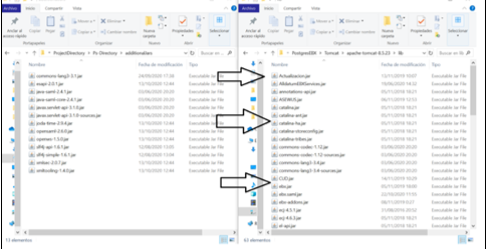
\includegraphics[width=0.7\textwidth]{Requerimientos/ConfiguracionLDAP-Bases/CL01.png}
        \caption{Información recibida por parte del lado del cliente}
    \end{figure}

    \item Lo cual permite conocer que existen 3 servidores donde se pueden encontrar los usuarios a autentificar, lo que lleva a crear una clase personalizada para gestionar los 3 directorios externos. La nueva implementación se aplicó dentro de la clase: com.orchestranetworks.ps.customDirectory.LdapDirectoryFactoryV3 que se encuentra dentro de la librería ps-directory.jar. 
    \begin{figure}[H]
        \centering
        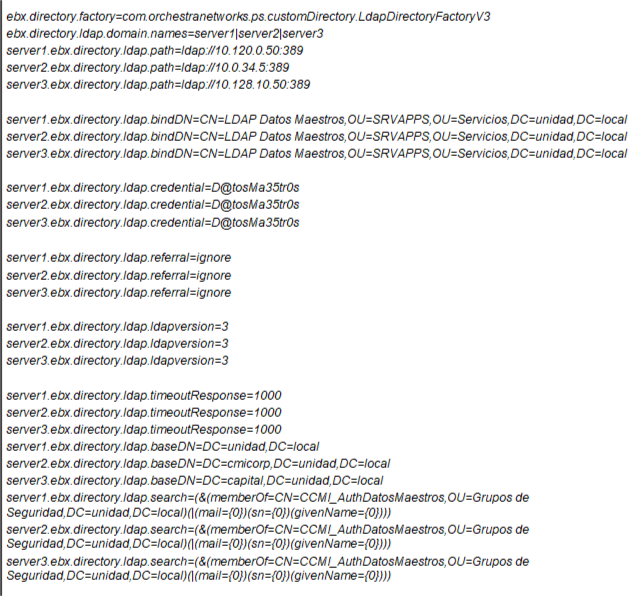
\includegraphics[width=0.7\textwidth]{Requerimientos/ConfiguracionLDAP-Bases/CL02.png}
        \caption{Gestión de los directorios externos mediante una clase personalizada}
    \end{figure}

    \item Lo siguiente es el properties utilizado para CMI: 
     \begin{figure}[H]
        \centering
        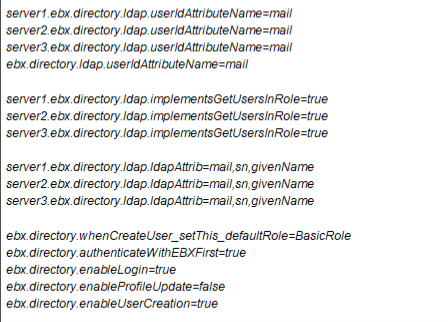
\includegraphics[width=0.5\textwidth]{Requerimientos/ConfiguracionLDAP-Bases/CL03.png}
        \caption{Archivo properties enfocado a CMI.}
    \end{figure}

\end{enumerate}


\section{Configuración de conexión a fuente de Datos}

\begin{enumerate}
    \item Para realizar una conexión a fuente de datos, es necesario estar dentro la perspectiva avanzada y dirigirse al icono de administración (llave inglesa). Dentro de éste se navegará en el menú desplegable y se accederá al área de intercambio de datos. 
     \begin{figure}[H]
        \centering
        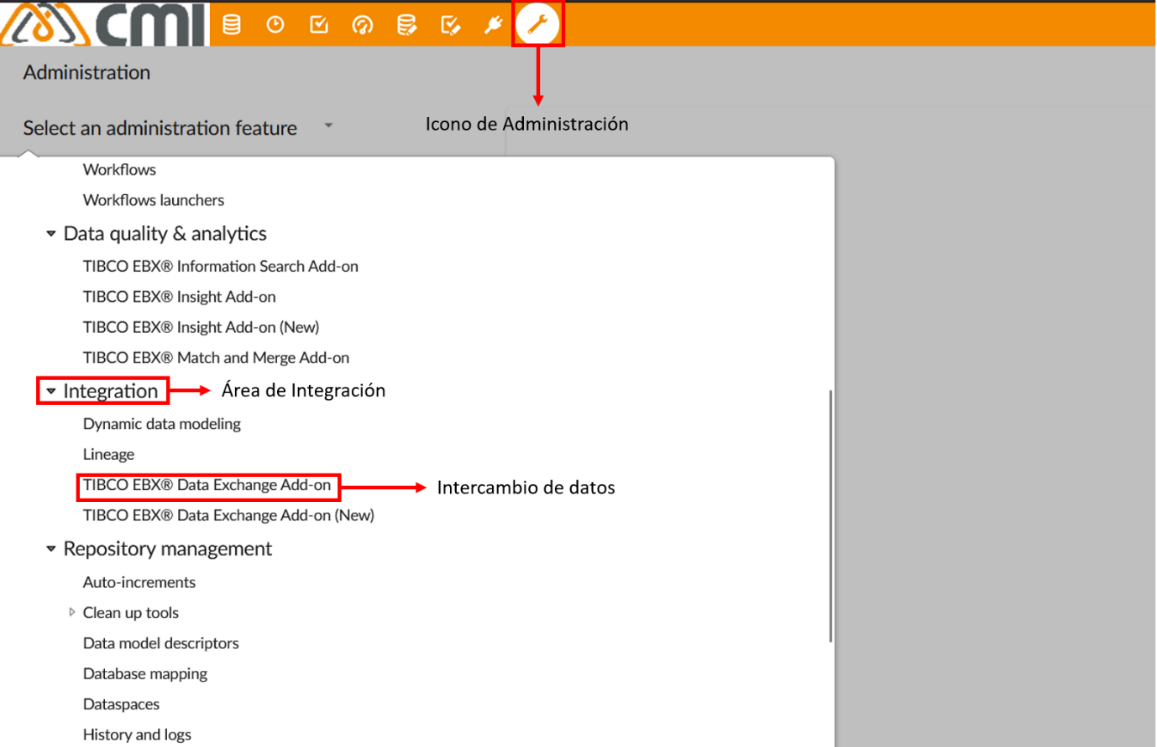
\includegraphics[width=0.5\textwidth]{Requerimientos/ConfiguracionLDAP-Bases/CL04.png}
        \caption{Dirección hacia Intercambio de datos dentro de TIBCO EBX}
    \end{figure}

    \item Dentro de esta área hay varias secciones disponibles, hay que enfocarse en la sección de datos de referencia donde se encontrará el apartado llamado “JDNI Data Source”; el cual contiene las conexiones actuales.
     \begin{figure}[H]
        \centering
        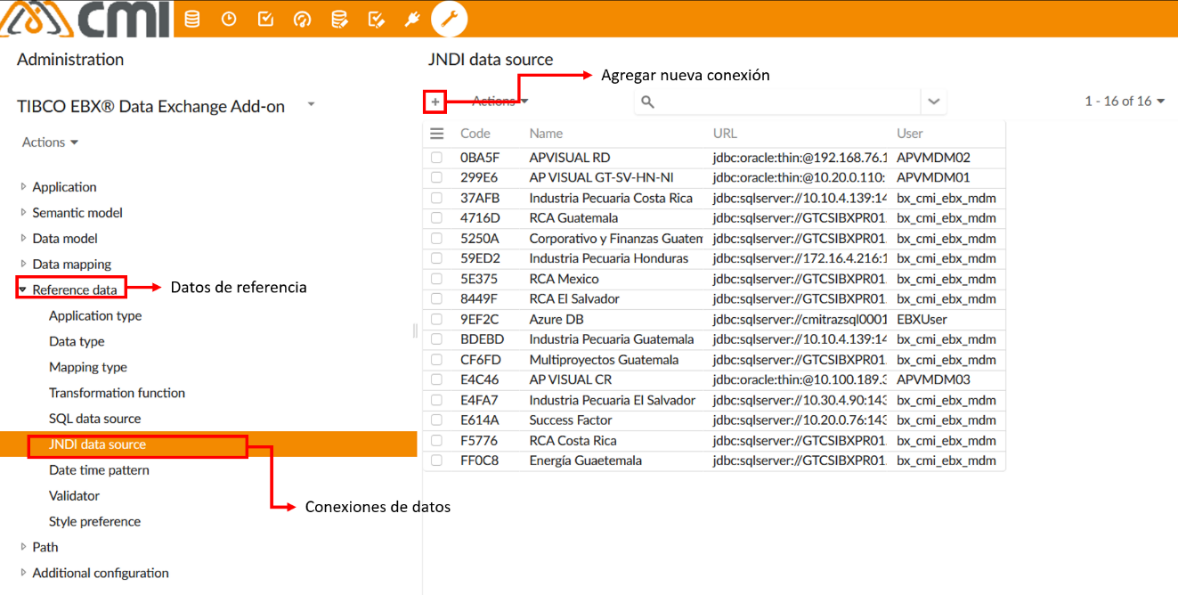
\includegraphics[width=0.5\textwidth]{Requerimientos/ConfiguracionLDAP-Bases/CL05.png}
        \caption{Conexiones actuales dentro de TIBCO EBX}
    \end{figure}

    \item Al agregar una nueva conexión se direccionará a otra pantalla en la cual se creará el registro para la conexión. Dentro de esta pantalla se aprecian los siguientes apartados: 

    \begin{itemize}
        \item Código es un identificador que se genera de manera automática. 
        \item Nombre es el cómo se identificará esta conexión a las demás.   
        \item URL de conexión para la base de datos. 
        \item Usuario asignado para acceder a la base de datos. 
        \item Contraseña de conexión a la base de datos.
    \end{itemize}

    \item Una vez llenados todos los apartados, se hace una prueba de conexión usando el botón “Test Connection”, para así obtener el siguiente mensaje y comprobar que la conexión se creó de manera correcta. 
     \begin{figure}[H]
        \centering
        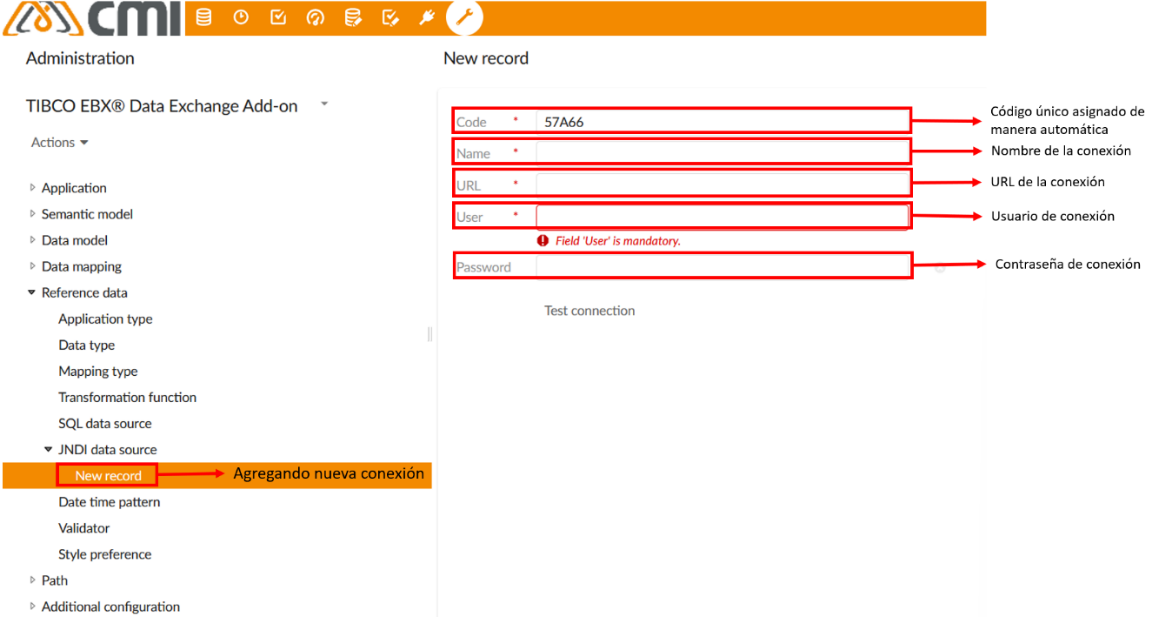
\includegraphics[width=0.5\textwidth]{Requerimientos/ConfiguracionLDAP-Bases/CL06.png}
        \caption{Mensaje de éxito en la prueba de conexión.}
    \end{figure}

    \item Después de obtener el mensaje exitoso de conectividad, se debe crear una relación entre la conexión y el modelo de datos que va a utilizar la conexión; para lo cual se ingresa al apartado de “SQL Data Source” donde se creará la relación. 
     \begin{figure}[H]
        \centering
        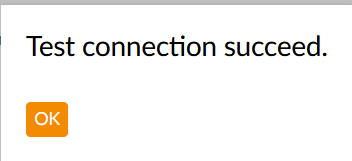
\includegraphics[width=0.5\textwidth]{Requerimientos/ConfiguracionLDAP-Bases/CL07.png}
        \caption{Relación entre conexión y modelo de datos.}
    \end{figure}
    
    \item Al crear una nueva relación se deben llenar los siguientes elementos: 
    \begin{itemize}
        \item \textbf{Código}, valor automático que proporciona la herramienta.
        
        \item \textbf{Nombre}, hace referencia al nombre que se le da a la conexión al momento de crearla. 
        \begin{figure}[H]
            \centering
            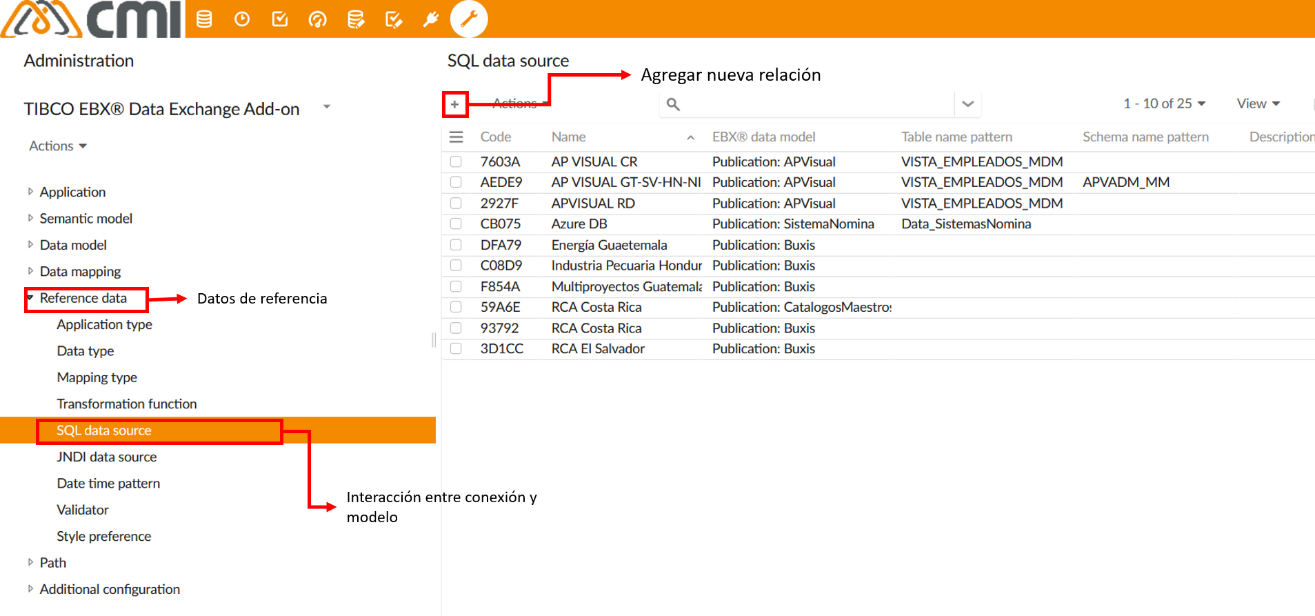
\includegraphics[width=0.5\textwidth]{Requerimientos/ConfiguracionLDAP-Bases/CL08.png}
            \caption{Ingreso de una nueva relación (código y nombre de conexión).}
        \end{figure}

        \item \textbf{Modelo de datos EBX}, es la referencia al modelo de datos donde se usará la conexión antes creada. 
        \begin{figure}[H]
            \centering
            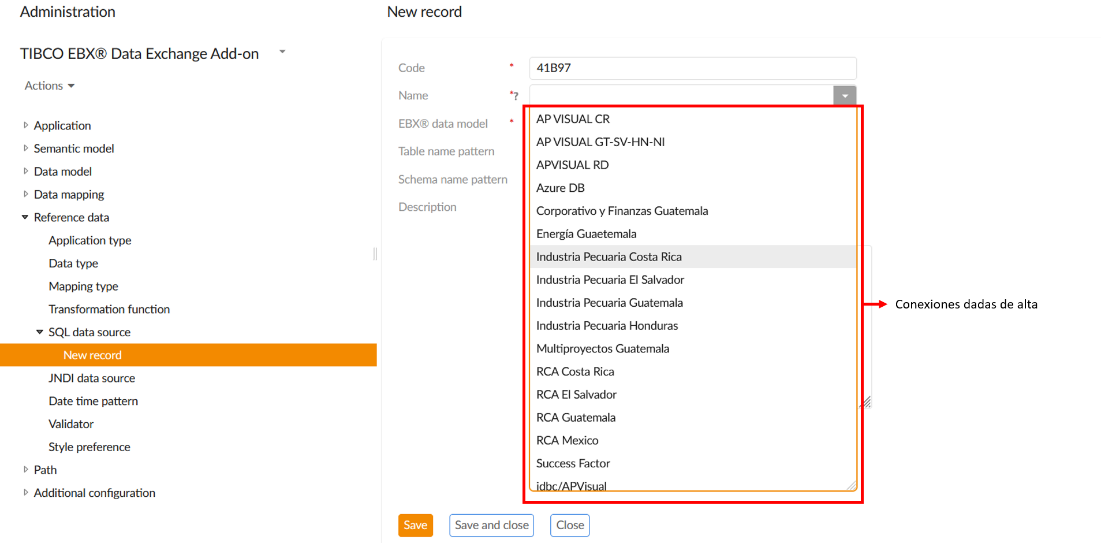
\includegraphics[width=0.5\textwidth]{Requerimientos/ConfiguracionLDAP-Bases/CL09.png}
            \caption{Modelo donde se usará la conexión}
        \end{figure}

        \item \textbf{Patrón de nombre de Tabla} (opcional), este campo ayuda a reducir las opciones de búsqueda dentro la conexión a una en específico o en su caso a diferentes. 
        
        \item \textbf{Patrón de nombre de Esquema} (opcional), este campo ayuda a reducir las opciones de búsqueda dentro la conexión a una en específico o en su caso a diferentes. 

        \item \textbf{Descripción}, si es necesario y por comodidad se le pueda dar una descripción a la relación creada. 
        \begin{figure}[H]
            \centering
            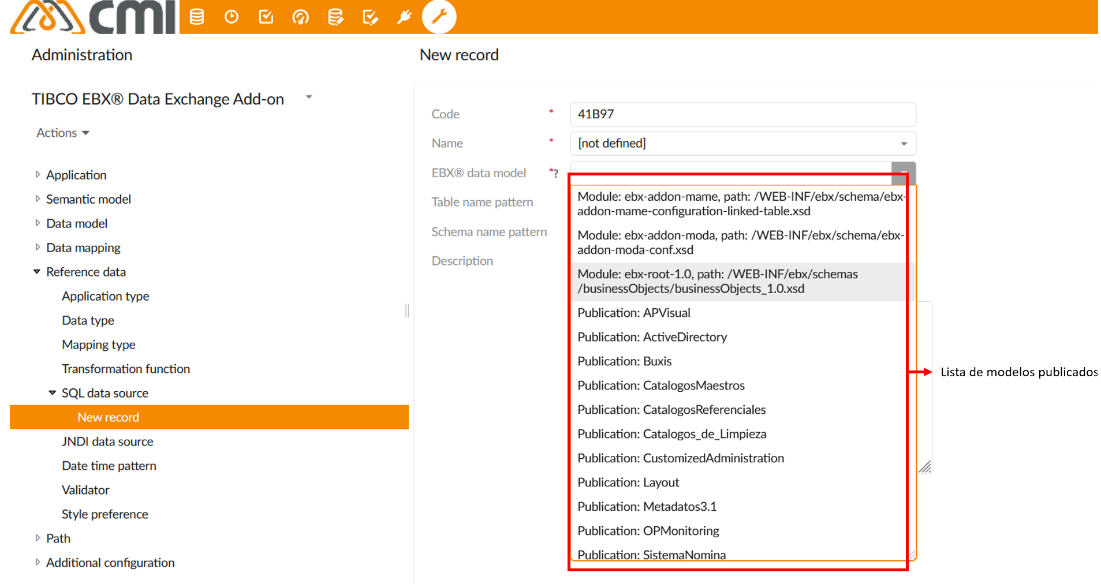
\includegraphics[width=0.5\textwidth]{Requerimientos/ConfiguracionLDAP-Bases/CL10.png}
            \caption{Vista completa de un nuevo registro sobre una nueva relación entre conexión y modelo de datos.}
        \end{figure}
    
    \end{itemize}
     
\end{enumerate}

%%%% ---------------- Acceso a metadatos técnicos y configuraciones de limpieza-----------

\section{Acceso a metadatos técnicos y configuraciones de limpieza}

Para encontrar los metadatos técnicos y funciones aplicadas a las reglas de calidad de los datos, se debe dirigir a la perspectiva avanzada de TIBCO EBX (habilitada únicamente para usuarios de tipo administrador) y dirigirse en la pestaña de \textbf{“Data”} en la parte superior izquierda de la pantalla. Posteriormente buscar dentro de los espacios de datos el espacio con el nombre \textbf{“[Metadata] Metadatos técnicos”}, seleccionando el dataset del mismo nombre.
\begin{figure}[H]
    \centering
    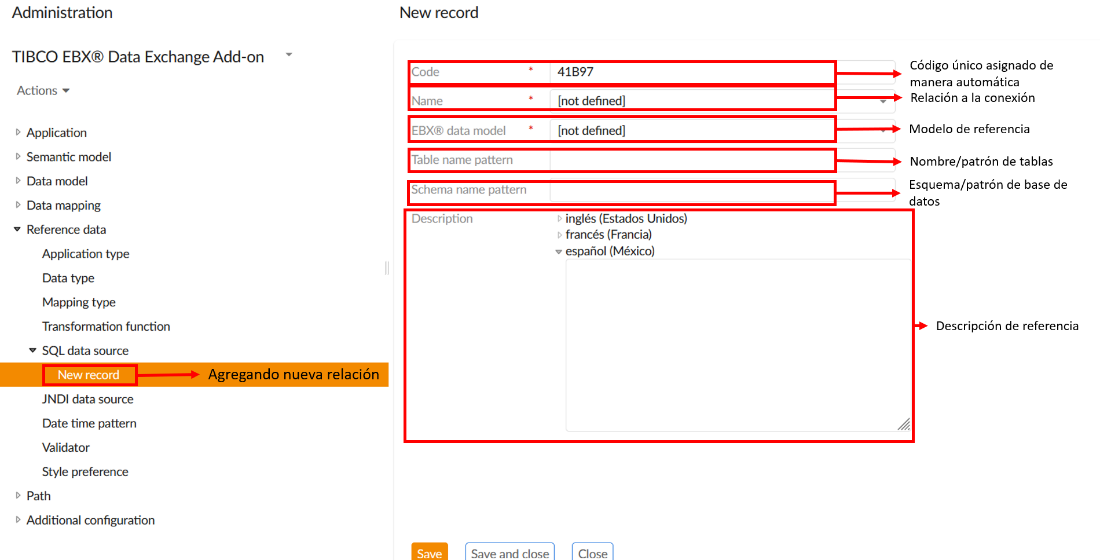
\includegraphics[width=0.8\textwidth]{Requerimientos/ConfiguracionLDAP-Bases/CL11.png}
    \caption{Espacio y conjunto de datos de los Metadatos técnicos.}
\end{figure}

Se desplegará del lado izquierdo de la pantalla una lista de opciones a elegir referentes a los metadatos técnicos del sistema de EBX. Dentro de estas opciones dar clic en la opción de \textbf{“Data Cleansing”}, la cual contiene los datos de referencia al proceso de calidad de los datos.

Dentro de esta opción se encontrarán 4 tablas disponibles:
\begin{figure}[H]
    \centering
    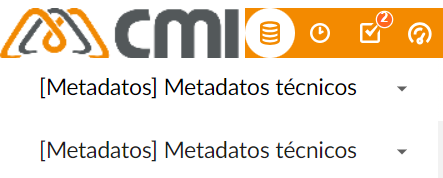
\includegraphics[width=0.8\textwidth]{Requerimientos/ConfiguracionLDAP-Bases/CL12.png}
    \caption{Tablas referentes a Data Cleansing}
\end{figure}

Ingresando en la tabla de “Function”, se encontrarán 5 columnas correspondientes al listado de funciones que se pueden utilizar en los procesos de limpieza con los que cuenta la herramienta actualmente. Estas columnas son:
\begin{enumerate}
    \item \textbf{ID:} Contiene el número entero auto incremental con el que se contabilizan las funciones ingresadas al sistema.
    
    \item \textbf{Name:} Contiene el nombre técnico que recibe la función.
    
    \item \textbf{Label:} Contienen los nombres o etiquetas con las que se podrá reconocer la función al momento de consumirla dentro del proceso de limpieza.
    
    \item \textbf{Description:} Tiene como objetivo resumir el objetivo que tiene la función analizada en concreto.
    
    \item \textbf{Return:} Contiene una descripción del resultado obtenido después de la realización de la función específica.

\end{enumerate}

\begin{figure}[H]
    \centering
    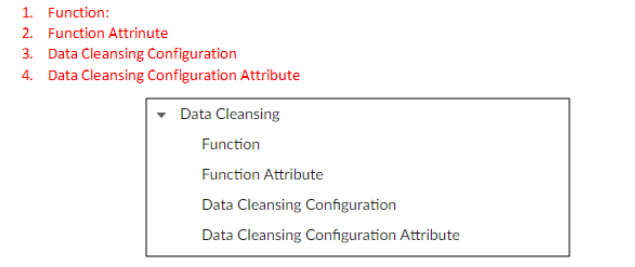
\includegraphics[width=0.8\textwidth]{Requerimientos/ConfiguracionLDAP-Bases/CL13.png}
    \caption{Ejemplos de funciones para el proceso de limpieza.}
\end{figure}

Al ingresar cualquier función de las enlistadas en dicha tabla se pueden observar dos pestañas de datos. \textbf{“Main/Principal”}, la cual contiene los datos desplegados que se encuentran expuestos en la vista principal de la tabla de Funciones; y \textbf{“Attributes”}, la que muestra los parámetros de entrada que serán solicitados al momento de consumir la función.

\begin{figure}[H]
    \centering
    \begin{minipage}[b]{0.45\textwidth}
    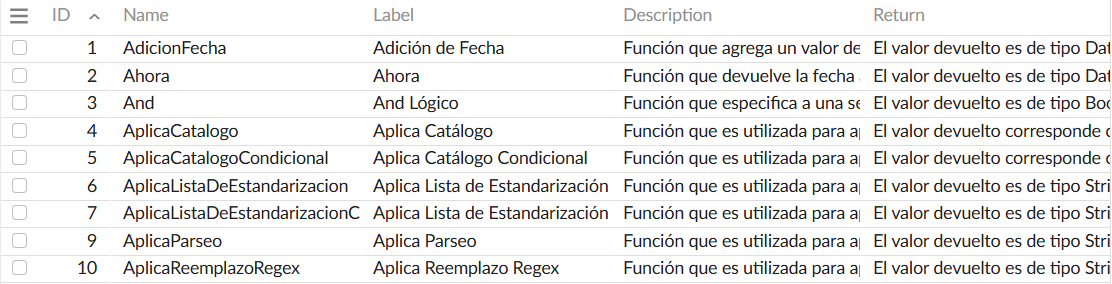
\includegraphics[width=\textwidth]{Requerimientos/ConfiguracionLDAP-Bases/CL14.png}
    \caption{Pestaña Principal de la Función.}
    \end{minipage}
    \begin{minipage}[b]{0.45\textwidth}
    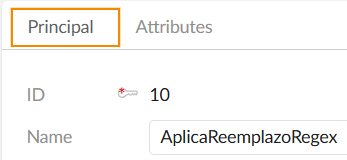
\includegraphics[width=\textwidth]{Requerimientos/ConfiguracionLDAP-Bases/CL15.png}
    \caption{Pestaña Attributes de la Función}
    \end{minipage}
\end{figure}

Ingresando a la tabla de \textbf{“Function Attribute”} se encuentran 8 columnas correspondientes a los atributos consumidos por las funciones contenidas en la tabla \textbf{“Function”}. Estas columnas son:
\begin{enumerate}
    \item \textbf{ID:} Contiene número entero auto incremental con el que se contabilizan los atributos ingresados al sistema.

    \item \textbf{Label:} Campo que contiene los nombres o etiquetas con los que se podrá reconocer el atributo al momento de consumirla dentro del proceso de limpieza.
    
    \item \textbf{Name:} Contiene el nombre técnico que recibe el atributo seleccionado.
    
    \item \textbf{Data Type:} Muestra el tipo de dato que consume el atributo seleccionado.
    
    \item \textbf{Description:} Su objetivo es resumir el objetivo del atributo analizado.
    
    \item \textbf{Internal:} Etiqueta descriptiva para diferenciar atributos similares dentro de la función.
    
    \item \textbf{Function:} Etiqueta de la función a la que pertenece el atributo seleccionado.
    
    \item \textbf{Function Name:} Nombre técnico de la función a la cual pertenece el atributo seleccionado.
    
\end{enumerate}

\begin{figure}[H]
    \centering
    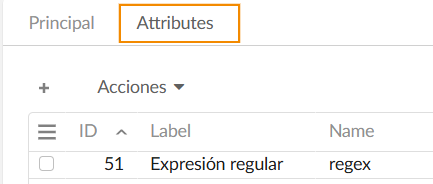
\includegraphics[width=0.8\textwidth]{Requerimientos/ConfiguracionLDAP-Bases/CL16.png}
    \caption{Ejemplo de atributos de funciones dentro de la tabla Fuction Attribute.}
\end{figure}

Si se ingresa a cualquier atributo relacionado con alguna función, en el campo \textbf{“Function”} se brindará un hipervínculo para consultar la función que consume a dicho atributo. Se puede acceder a la información de la función dando clic en el símbolo de flecha que se encuentra a la derecha del campo.
\begin{figure}[H]
    \centering
    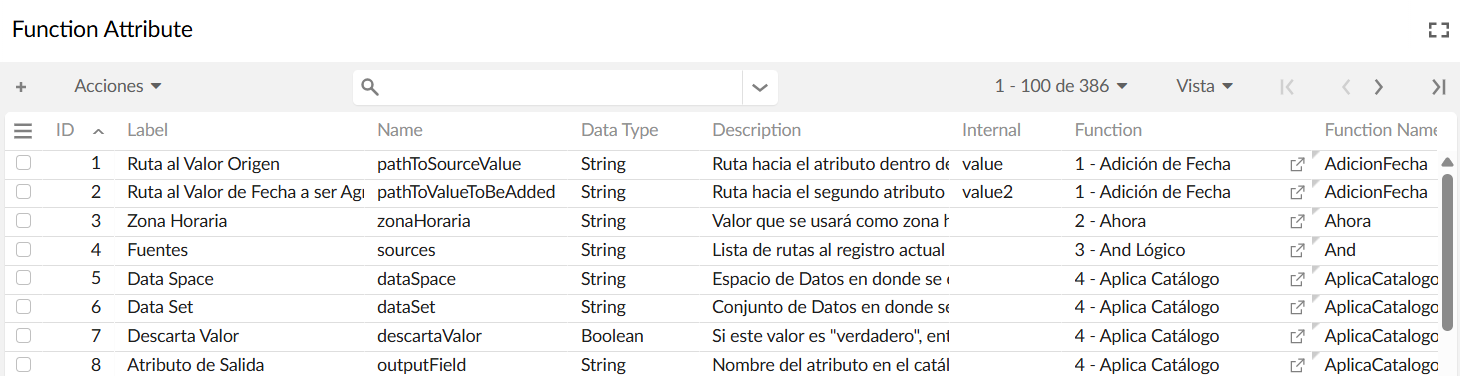
\includegraphics[width=0.8\textwidth]{Requerimientos/ConfiguracionLDAP-Bases/CL17.png}
    \caption{Campo Function dentro de un registro de atributo.}
\end{figure}

Al seleccionar la tabla de \textbf{“Data Cleansing Configuration”} se encontrará una tabla la cual lleva a las configuraciones de limpieza de cada entidad dentro de TIBCO EBX que tenga un proceso que requiera uso de estas funciones dentro de CMI.
\begin{figure}[H]
    \centering
    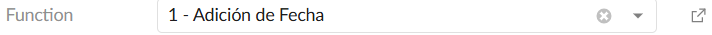
\includegraphics[width=0.8\textwidth]{Requerimientos/ConfiguracionLDAP-Bases/CL18.png}
    \caption{Ejemplo de registros configurados en Data Cleansing Configuration.}
\end{figure}

Una vez se va a crear una nueva configuración de limpieza, se podrá apreciar en primera instancia la pestaña de \textbf{“Main”}; la cual contendrá los datos de la tabla a la que se hará referencia (Espacio de datos, Conjunto de datos y Tabla), en caso de que se necesiten enviar los resultados a una segunda tabla. De igual forma, se ingresarán los datos requeridos (Espacio de datos, conjunto de datos y tabla objetivos) y los datos del espacio de monitoreo de proceso para este proceso de limpieza especifico.
\begin{figure}[H]
    \centering
    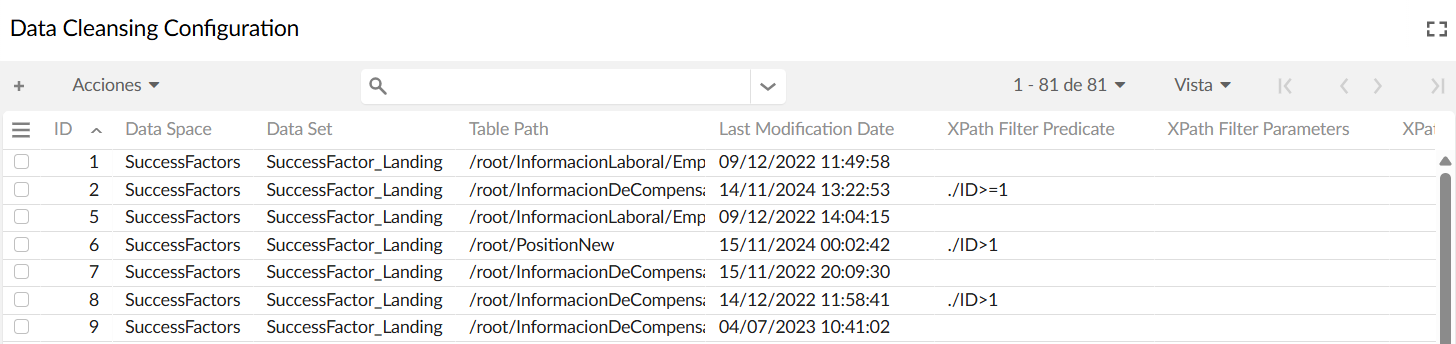
\includegraphics[width=0.8\textwidth]{Requerimientos/ConfiguracionLDAP-Bases/CL19.png}
    \caption{Ejemplo de configuración de pestaña Main.}
\end{figure}

Una vez se guarda la configuración de la pestaña \textbf{“Main”} se habilita la pestaña de \textbf{“Attributes”}, en la cual se encuentran las configuraciones de limpieza para todos y cada uno de los campos creados para el proceso de limpieza de datos. Dicha vista consta de 9 columnas las cuales son:

\begin{enumerate}
    \item \textbf{ID:} Contiene número entero auto incremental con el cual se identifican los campos de esta tabla.
    
    \item \textbf{Position:} Al ser un proceso lineal de ejecución, este campo proporciona el orden con el que se realizarán las funciones durante el proceso de limpieza.
    
    \item \textbf{Attribute:] Ruta al campo sobre el que se realizará la función.
    
    \item \textbf{Data Type:} Tipo de dato del campo sobre el que se realizará la función.
    
    \item \textbf{Description:] Descripción del campo, aquí se coloca cual es el objetivo del campo, así como su funcionalidad durante el proceso de limpieza.
    
    \item \textbf{Result:} Resultado de la función aplicada para un parámetro de ejemplo.
    
    \item \textbf{Function:} Función que se llevará a cabo en este campo.
    
    \item \textbf{Parameters:} Aquí se encuentran los atributos de la función seleccionada para el campo seleccionado.

    \item \textbf{Last Modification Date:} Fecha en la cual se realizó la última modificación a la función de cada campo.
\end{enumerate}
\begin{figure}[H]
    \centering
    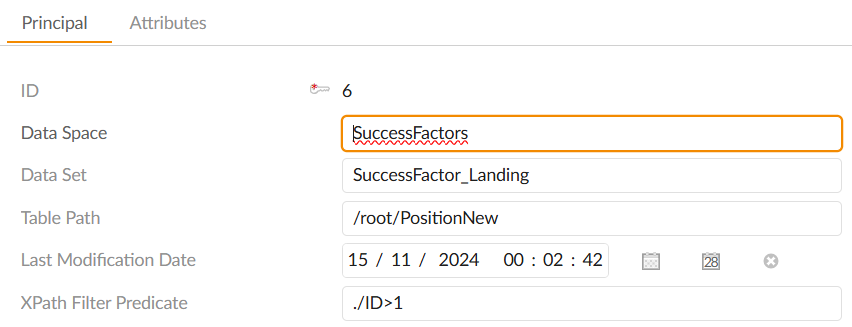
\includegraphics[width=0.8\textwidth]{Requerimientos/ConfiguracionLDAP-Bases/CL20.png}
    \caption{. Ejemplo de configuración de pestaña Attributes}
\end{figure}

Al ingresar a cada uno de los campos, se desplegará a mayor detalle los campos anteriormente mencionados, desplegando los atributos necesarios para las funciones seleccionadas. De igual forma, en el campo de \textbf{“Function”} se da acceso a un hipervínculo localizado en el símbolo al final del campo (en forma de flecha) con el cual se redireccionará al detalle de la función seleccionada.